\newpage
\section{Polarización del punto Q}
\sangria{En este trabajo implementamos un transistor JFET en configuración fuente común, para aplicar el modelo MES, en esta oportunidad implementamos el modelo con autopolarización. Nuestros datos iniciales fueron $V_{DD}= 12V$ $R_G=1M\Omega$, además contabamos también con los datos del punto Q ya predefinidos $I_{DQ}=\frac{I_{DSS}}{2}$ y $V_{DSQ}=\frac{V_{DD}}{2}$}
\sangria{Primero revelamos la curva de $I_{DSS}$, para luego calcular $R_S$ $R_D$, la curva relevada fue la siguiente.}
\midTitle{blue}{Mediciones de $I_{DSS}$ Obtenidas}{}
\begin{center}
\setlength{\tabcolsep}{4pt}
\captionof{table}{Mediciones de $I_{DSS}$ en función de $V_{DS}$.}
\begin{tabular}{|
>{\columncolor[HTML]{FFCCC9}}c |
c | c |}
\hline
\rowcolor[HTML]{FFFFC7}
\textbf{$V_{DS}$ (V)} & \textbf{$I_{DSS}$ (mA)} & \textbf{Diferencia (\%)} \\ \hline
0.200 & 2.112 & - \\ \hline
0.440 & 4.530 & 114.5 \\ \hline
0.600 & 5.500 & 21.4 \\ \hline
0.820 & 6.050 & 10.0 \\ \hline
1.015 & 6.390 & 5.6 \\ \hline
1.235 & 6.560 & 2.7 \\ \hline
1.402 & 6.650 & 1.4 \\ \hline
1.650 & 6.742 & 1.4 \\ \hline
1.815 & 6.787 & 0.7 \\ \hline
2.020 & 6.834 & 0.7 \\ \hline
2.200 & 6.853 & 0.3 \\ \hline
2.450 & 6.893 & 0.6 \\ \hline
2.609 & 6.913 & 0.3 \\ \hline
2.830 & 6.942 & 0.4 \\ \hline
\end{tabular}
\end{center}

\begin{figure}[H]
    \centering
    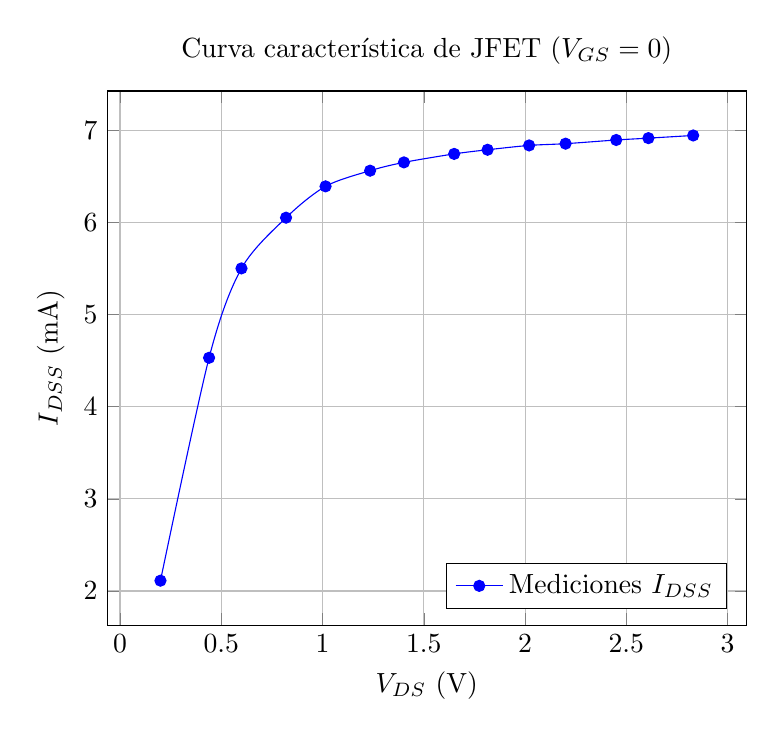
\begin{tikzpicture}
    \begin{axis}[
        title={Curva característica de JFET ($V_{GS} = 0$)}, % Título del gráfico
        xlabel={$V_{DS}$ (V)},          % Etiqueta eje X
        ylabel={$I_{DSS}$ (mA)},        % Etiqueta eje Y
        grid=major,                   % Grilla principal
        legend pos=south east,        % Posición de la leyenda (esquina inf. derecha)
        width=0.8\textwidth,          % Ancho del gráfico
    ]

    \addplot [
        smooth,     % Suaviza la línea que une los puntos
        mark=*,     % Pone un marcador en cada punto de la tabla
        blue,       % Color de la línea
    ]
    % Aquí van los datos Vds (x) e Idss (y) de tu tabla
    coordinates {
        (0.200, 2.112)
        (0.440, 4.530)
        (0.600, 5.500)
        (0.820, 6.050)
        (1.015, 6.390)
        (1.235, 6.560)
        (1.402, 6.650)
        (1.650, 6.742)
        (1.815, 6.787)
        (2.020, 6.834)
        (2.200, 6.853)
        (2.450, 6.893)
        (2.609, 6.913)
        (2.830, 6.942)
    };
    \addlegendentry{Mediciones $I_{DSS}$}

    \end{axis}
    \end{tikzpicture}
    \caption{Curva de salida $I_D = f(V_{DS})$ para $V_{GS} = 0$.}
    \label{fig:curva_jfet}
\end{figure}
\newpage
\subsubsection{Cálculos del punto Q}
\sangria{Una vez revelada la curva, el valor de $I_{DSS}$ se extrajo a partir de las diferencias porcentules del mismo valor, el valor elejido fue: $I_{DSS} = 6,650mA$, ya que la diferencia porcentual con el valor anterior fue del $1.4\%$, el valor de tensión en este punto se denomina $V_{GSoff}$ y es de $V_{GSoff}=1,402V$}

$$I_{DQ}=\frac{I_{DSS}}{2}$$
$$I_{DQ}=\frac{6,650mA}{2}$$
$$I_{Q}=3,325mA$$

\sangria{El siguiente paso fue calcular las resistencias para situar el punto Q, para esto primero obtenemos el valor de $V_{GS}$ para luego obtener $R_S$ y finalmente obtenemos $R_D$. Las ecuaciones de las cuales obtenemos estos valores son las siguiente:}

$$i_{D}=I_{DSS}*(1-\frac{V_{GS}}{V_{GSoff}})^2$$
$$V_{GS}=-i_{D}*R_{S}$$
$$V_{DD}=i_{D}*(R_{S} + R_{D})+V_{DS}$$

\sangria{De la primera ecuación despejamos $V_{GS}$, como nos encontramos en el punto Q, podemos sustituir $i_D$ por $I_{DQ}$ y queda:}
$$V_{GS}=(\sqrt{\frac{i_D}{I_{DSS}}}-1)*-V_{GSoff}$$
$$V_{GS}=(\sqrt{\frac{I_{DQ}}{I_{DSS}}}-1)*-V_{GSoff}$$
$$V_{GS}=(\sqrt{\frac{I_{DSS}}{2*I_{DSS}}}-1)*-V_{GSoff}$$
$$V_{GS}=(\sqrt{\frac{1}{2}}-1)*-V_{GSoff}$$
$$V_{GS}=-0,4106V$$

\sangria{Con este dato podemos obtener $R_S$ a partir de la segunda ecuación:}
$$R_S={\large{|}\frac{-V_{GS}}{I_{DQ}}}\large{|}$$
$$R_S=123,48\Omega$$
\sangria{Ya con este valor podemos calcular $R_D$}
$$$$
